\noindent
\begin{tcolorbox}[colframe=black,width =7cm,colback=gray!20,arc=0pt]
\centering {\sc {\bf Questão 03}}
\end{tcolorbox}

Para modelar um canal de comunicações digitais via rádio usa-se, comumente, o chamado “modelo de dois raios”, ilustrado na figura a seguir.
Neste modelo, o sinal $x(n)$ recebido em R\textsubscript{X} é modelado como o resultante da soma de duas versões do sinal $s(n)$ transmitido por T\textsubscript{X}, cada versão multiplicada por certo ganho e atrasada de certo número de amostras.
Evidentemente, a soma dessas versões defasadas provoca uma distorção no sinal transmitido.
Para compensá-la necessita-se de incorporar um filtro ao receptor que funcione como sistema inverso ao canal.
É o chamado processo de desconvolução.
Para efeito de simplificação, costuma-se atribuir atraso zero e ganho unitário ao primeiro raio.
Se temos então atraso $N_0$ e ganho a para o segundo raio, o modelo do canal é dado por $H(z) = 1 + az^{-N_0}$.
Queremos calcular o filtro de desconvolução $W(z)$, com $M$ coeficientes, por dois métodos:
o método de Wiener, largamente discutido na aula;
e o método de Robinson, que remonta à aplicação de predição linear na desconvolução sísmica.

\begin{figure}[h!]
    \centering
    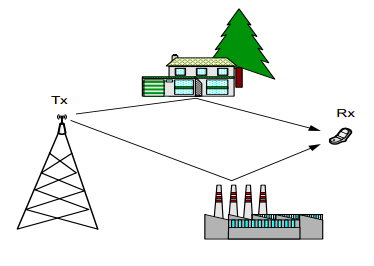
\includegraphics{../img/03/enunciado}
\end{figure}

\begin{enumerate}[label={\bf \roman*:},series=exerc,align=left]
    \item Indique a formulação de Wiener para a solução do problema, isto é, a equação matricial que fornece os coeficientes ótimos $\mathbf{w} = [w_0, w_1, \dots, w_{M-1}]^\T$, do filtro de desconvolução, explicitando claramente as grandezas envolvidas.

    Pelo canal proposto, o sinal recebido em R\textsubscript{X} é $x(n) = s(n) + as(n-N_0)$.
    Os termos da matriz de autocorrelação de $\mathbf{x}$, para $M$ termos, são:
    \begin{align*}
        r(k) &= E[x(n)x(n-k)] \\
        &= E[(s(n)+as(n-N_0))(s(n-k)+as(n-k-N_0)] \\
        &= E[s(n)s(n-k)] + aE[s(n-N_0)s(n-k)] + aE[s(n)s(n-(k+N_0))] + a^2E[s(n-N_0)s(n-(k+N_0))]
    \end{align*}
    Cada um dos termos se refere à correlação entre amostras do sinal $s(n)$.
    Essa correlação é nula, para amostras diferentes.
    Então:
    \begin{align*}
        E[s(n)s(n-k)] &= \begin{cases}
                            1 \quad k=0 \\
                            0 \quad \text{caso contrário}
                        \end{cases} \\
        E[s(n-N_0)s(n-k)] &= \begin{cases}
                                1 \quad k=N_0 \\
                                0 \quad \text{caso contrário}
                            \end{cases} \\
        E[s(n)s(n-(k+N_0))] &= 0 \\
        E[s(n-N_0)s(n-(k+N_0))] &= \begin{cases}
                                      1 \quad k=0 \\
                                      0 \quad \text{caso contrário}
                                  \end{cases}
    \end{align*}
    Assim, os termos são:
    \begin{align*}
        r(0) &= 1+a^2 \\
        r(N_0) &= a \\
        r(k) &= 0 \qquad \forall k \neq 0 \text{ e } k \neq N_0
    \end{align*}
    Por exemplo, para $M=3$ e $N_0=2$, a matriz resultante é
    \begin{equation*}
        \mathbf{R} = \left[  \begin{matrix}
                        1+a^2 & 0 & a \\
                        0 & 1+a^2 & 0 \\
                        a & 0 & 1+a^2
                    \end{matrix} \right]
    \end{equation*}
    Falta encontrarmos o vetor de correlação cruzada entre o sinal recebido, $x(n)$ e o sinal desejado, $d(n)$.
    É uma escolha natural desejarmos obter o sinal original, logo $d(n) = s(n)$.
    \begin{align*}
        p(k) &= E[d(n)x(n-k)] \\
        &= E[s(n)x(n-k)] \\
        &= E[s(n)s(n-k)] + aE[s(n)s(n-(k+N_0))]\\
        E[s(n)s(n-k)] &= \begin{cases}
                            1 \quad k=0 \\
                            0 \quad \text{caso contrário}
                        \end{cases} \\
        E[s(n)s(n-(k+N_0))] &= 0 \\
    \end{align*}
    Dessa forma, seguindo o mesmo exemplo, $\mathbf{p} = \left[\begin{matrix} 1 \\ 0 \\  0 \end{matrix} \right]$.
    Podemos, então, fornecer a solução de Wiener para o problema da desconvolução:
    $\mathbf{w_{opt}} = \mathbf{R}^{-1}\mathbf{p}$.


    \item Indique a formulação de Robinson para a solução do problema, isto é, a equação matricial que fornece os coeficientes ótimos de predição $\mathbf{w_f} = [w_{1f}, w_{2f}, \dots, w_{(M-1)f}]^\T$, do filtro de desconvolução, explicitando claramente as grandezas envolvidas.

    Já para a formulação de Robinson, uma desconvolução não-supervisionada, não temos, teoricamente, acesso ao sinal desejado $s(n)$ para obtermos o filtro de Wiener ótimo.
    Definimos, então, o erro de predição:
    \begin{equation*}
        e_f(n) = x(n) - \sum_{k=1}^{K}w_{kf} x(n-k)
    \end{equation*}
    Queremos que o erro de predição seja o menor possível: $\text{min} \; E[|e_f(n)|^2]$.
    A solução trivial, $w_{kf} = 0 \quad \forall k$ pode ser evitada introduzindo algumas restrições.
    Tais restrições podem ser obtidas impondo que o erro é descorrelacionado de amostras anteriores: $E[e_f(n)x(n-l)] = 0 \quad l \geq 1$.
    \begin{align*}
        E[e_f(n)x(n-l)] &= 0 \\
        \sum_{k=1}^{K} E[x(n-k)x(n-l)] a_k &= E[x(n)x(n-l)] \quad l = 1, 2, \dots, K
    \end{align*}
    Suponha agora o caso bem simples de $a = 0.625$ e $N_0 = 1$.
    \item Obtenha a solução de Wiener para $M = 9$
    Em seguida, trace a resposta em frequência, módulo e fase, do sistema combinado $H(z)W(z)$.

    Para a solução de Wiener, obtemos o seguinte conjunto de coeficientes:
    \begin{equation*} \mathbf{w} = \left[\begin{matrix}1.0\\-0.625\\0.39\\-0.243\\0.151\\-0.0932\\0.0561\\-0.0316\\0.0142\end{matrix}\right] \end{equation*}
    E a resposta do sistema $H(z)W(z)$:
    \begin{figure}[h!]
        \centering
        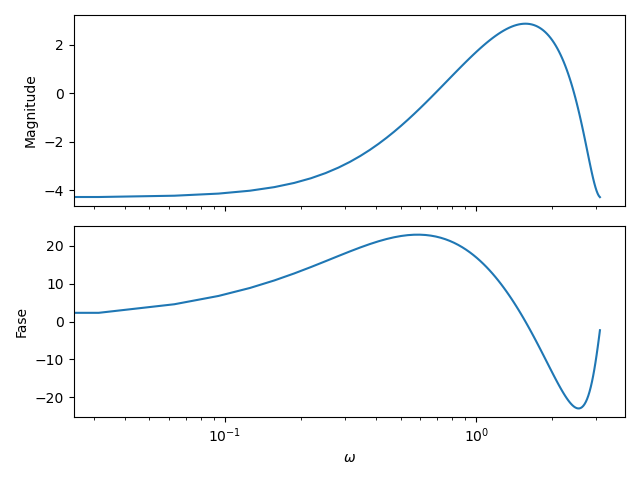
\includegraphics{../img/03/Wiener_Bode_0_625.png}
    \end{figure}

    \item Obtenha também a solução via predição linear para $M = 9$.
    Em seguida, trace a resposta em frequência, módulo e fase do sistema combinado $H(z)Wf(z)$.
    Compare com a do item anterior.

    \item Repita os itens anteriores para $a = 1.6$.
    Faça uma análise de seus resultados.

    Para o filtro de Wiener, com $a=1.6$ obtemos um outro conjunto de coeficientes:
    \begin{equation*} \mathbf{w} = \left[\begin{matrix}0.391\\-0.244\\0.152\\-0.095\\0.0591\\-0.0364\\0.0219\\-0.0123\\0.00554\end{matrix}\right] \end{equation*}
    E a resposta do sistema $H(z)W(z)$:
    \begin{figure}[h!]
        \centering
        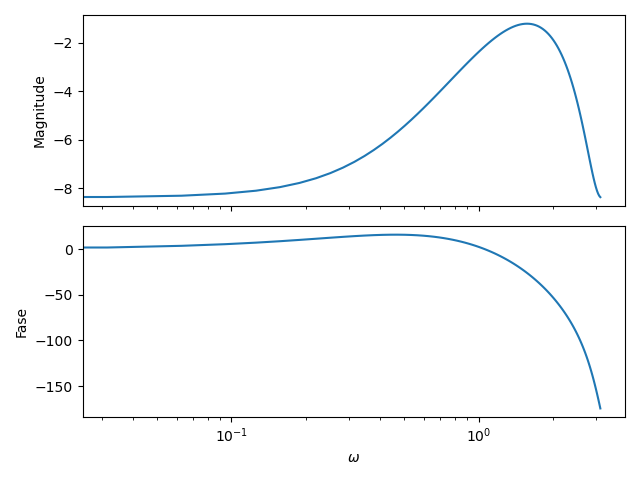
\includegraphics{../img/03/Wiener_Bode_1_6.png}
    \end{figure}

    Observe que, para altas frequências, a fase da resposta ultrapassa os 180 graus, o que leva a erros de decodificação.
    Foi observada uma taxa de erro em torno de 25\% para este canal.
    Algumas simulações a mais foram feitas e chegou-se à conclusão de que se $a<1$, a taxa de erro é nula, ou seja, o receptor consegue recuperar completamente o sinal original transmitido.
\end{enumerate}